\documentclass{bmvc2k}

\usepackage{subcaption}
%\usepackage{subfigure}
%\captionsetup{compatibility=false}
% \usepackage{graphicx}

%% Enter your paper number here for the review copy
\bmvcreviewcopy{??}

\title{Topological Analysis of Neural Network Transfer function}

% Enter the paper's authors in order
% \addauthor{Name}{email/homepage}{INSTITUTION_CODE}
\addauthor{Yogesh}{yogesh.kochar@iiitb.org}{1}
\addauthor{Sunil Kumar Vengalil}{sunilkumar.vengalil@iiitb.ac.in}{1}
\addauthor{Neelam Sinha}{neelam.sinha@iiitb.ac.in}{1}

% Enter the institutions
% \addinstitution{Name\\Address}
\addinstitution{
 International Institute of Information Technology\\
 Bangalore\\
 India
}


\runninghead{Student, Prof, Collaborator}{BMVC Author Guidelines}

% Any macro definitions you would like to include
% These are not defined in the style file, because they don't begin
% with \bmva, so they might conflict with the user's own macros.
% The \bmvaOneDot macro adds a full stop unless there is one in the
% text already.
\def\eg{\emph{e.g}\bmvaOneDot}
\def\Eg{\emph{E.g}\bmvaOneDot}
\def\etal{\emph{et al}\bmvaOneDot}

%-------------------------------------------------------------------------
% Document starts here
\begin{document}

\maketitle

\begin{abstract}
In Spite of the tremendous success of deep neural networks for solving complex tasks in domains like computer vision, speech recognition and natural language processing,  there has been little work on understanding the dynamics of the training process and also the working of a trained model. In this study, we analyze desired characteristics of the transfer function of each layer, and hence  the whole network,  based on the topological transformations of the space of training samples. We introduce a new family of activation functions that provides faster convergence for classification tasks. Based on our empirical results, we also propose a novel method for pruning and reducing the size of a trained model. We performed  experiments on previously studied, synthetic binary classification datasets with complex topology using Multi Layer Perceptron.We use betti numbers to quantify topological complexity and our experimental results show that the proposed activation function results in much faster convergence and the betti number reduces at a faster rate across layers with the proposed activation function. We verified our results on popular image classification datasets like fashion MNIST, CIFAR-10 and cat-vs-dog classification datasets by running experiments using Convolutional Neural Networks.
\end{abstract}

%-------------------------------------------------------------------------
\section{Introduction}
\label{sec:intro}
Deep neural networks have become the default choice for solving many tasks, which was otherwise either partially solved or not solved at all,  in domains like computer vision, speech and natural language processing where a lot of data is available. However, choosing the right architecture (like the  selection  of hyper parameters activation function, number of layers and number of units per layer)  for a specific task is mostly based on trial and error or based on the previous empirical results. The transfer function of each layer and the entire neural network is just treated as a complex, unknown and nonlinear function parameterized by weights and biases. Not much work has been done in identifying the impact of various favourable and unfavourable characteristics of this transfer function.

In this study we investigate some of the  desired characteristics a neural network architecture should have for solving a classification task. We derive our results based on the topology of the space of training data and how this topology changes as data is transformed by each layer.

Topology is a field of mathematics that studies the shape of objects and associated invariances like connectedness, number of holes etc.  It is observed that many real datasets when viewed as point cloud in a high dimensional space follow  certain topology. For example the study  in \cite{carlsson2008local} shows that the image patches obtained from natural images follow the topology of a Klein bottle. Topological Data Analysis\cite{carlsson2009topology}\cite{chazal2017introduction} uses topological tools ( like persistent topology ) for analysing point cloud dataset in order to identify and characterize underlying structures in a dataset.

Most of the existing work on the analysis of a trained model is limited to either looking at the learned weights and feature maps of each layer, with the goal of reusing these features across tasks, or techniques like Class activation map ( or saliency map\cite{meng2019class}  where the intention is to identify the relevant feature of input that is responsible for producing the output.  In their recent study, Gregory et. al. \cite{naitzat2020topology}  quantifies topological complexity using Betti numbers. They observe that topological changes to data across layers of a network remain robust under different instances of training. They further observe that, compared to smooth activation functions like sigmoid and tanh, non-homeomorphic activation functions like ReLU helps in changing the topology of data faster.

Our work is motivated by \cite{naitzat2020topology} where the transfer function of each layer is looked at based on  how the layer changes the topology of the data. Most real world datasets have non-trivial complex topology, and in order to perform classification each layer of the neural network transforms the entire space of data to a simpler topology. This leads us to the conclusion that in order to achieve classification, each layer of the neural networks should be able to change the topology of data and hence we need a non-homeomorphic transformation at each layer. This is achieved by activation functions with discontinuity like Relu. We followed the approach in \cite{naitzat2020topology} and used betti numbers to quantify  topological complexity of the point cloud dataset.

In addition to the above insight that the activation function should be non-homeomorphic, we also hypothesize that a many-to-one transfer function can help to bring samples from the same class closer in the transformed space( See appendix A for a skeleton of proof). Based on this hypothesis, we introduce a new activation function with multiple many-to-one regions and multiple discontinuities. Results of our experiments show that, with the proposed activation function the network converges faster as compared to commonly used activation functions like ReLU and sigmoid. It is also seen that the betti number, computed using persistent homology \cite{naitzat2020topology} reduces faster when with the proposed activation function.

The major contributions of our paper are:
\begin{enumerate}
\item We provide new guidelines for designing  activation functions for supervised classification tasks. We illustrate the guideline by proposing a  new family of activation functions.
\item We propose an easy technique for neural network pruning (i.e reducing the parameters in a trained model without significant decrease in accuracy) using betti numbers computed on the output feature space of each layer.
\end{enumerate}

\section{Related Work}
\section{Proposed Method}
\subsection{Problem Formulation}
We restrict our analysis to the task of supervised classification of  $3$-dimensional synthetic datasets using Multi Layer Perceptron(MLP ) and classification of images using Convolutional Neural Network. The classification task can be viewed as a many-to-one mapping, $f:R^d \mapsto \{c_1, c_2, \ldots c_k\}$  ( $f:R^{H \times W} \mapsto \{c_1, c_2, \ldots c_k\}$  in case of images). We denote the domain of the mapping with a discrete set $X$ with finite number of samples i.e  $X = \{x_1, x_2, x_3,\ldots x_n\}$.
The set of all samples $X$ form a point cloud dataset on $d$-dimensional space ($d=H \times W$ in case of image of height $H$ and width $W$).
The function $f$ is a composition of multiple functions, $g_l$, where $1 \leq l \leq L $ and each $g_l$ refers to the transfer function of layer $l$ and $L$ is the total number of layers in the neural network. As detailed in \cite{naitzat2020topology},  for classification task a non-homeomorphic transfer function is required for each layer as it can change the topology of point cloud dataset. In order to achieve classification one needs to change the topology from an initial complex topology to a simple and contractible topology for each class. Another important characteristic of layer transfer function is that each layer reduces the dimensionality of the input data.

Our study focuses on two important aspects of neural network design.
\begin{enumerate}
\item Design of an optimum non-linear activation function for supervised classification task. See subsection \ref{activation_function_design}  below.
\item Propose an easy technique for neural network pruning (i.e reducing the parameters in a trained model without significant decrease in accuracy) using betti numbers computed on the output feature space of each layer. See subsection \ref{network_pruning} for details.
\end{enumerate}
\subsection{Dataset}
We use two $3$-dimensional simulated datasets, nine ring dataset and nine sphere dataset used in \cite{naitzat2020topology}. The  nine ring dataset, as shown in Figure \ref{nine_ring_dataset},  consists of two classes of data,  colored Green and Red, interlocked together. The nine sphere dataset consists of nine Green spheres and 18 Red Spheres enclosing each other as shown in Figure \ref{nine_sphere_dataset}. Both the datasets contain 16000 samples for training and 2000 samples for testing.

We also performed experiments and provide results on the following real datasets:
\begin{enumerate}
\item Cat-Dog dataset in Kaggle - The dataset consists of  images of size $32 \times 32$. The dataset is divided into training and testing sets, with 8000 training images and 2000 testing images,  each set with an equal number of images of cats and dogs.
\item Fashion Minst - The dataset consists of 70,000 grayscale images of size $28 \times 28$ with 10 different categories. The dataset is divided into training and testing sets, with 60,000 training images and 10,000 test images.
\item CIFAR-10 - The dataset consists of 60,000 colour images of size $32 \times 32$ with 10 different categories. Each category consists of 6000 images. The dataset is divided into training and testing sets, with 50,000 training images and 10,000 test images.
\end{enumerate}

Some sample images from each of the above datasets are shown in Figure 2, Figure 3 and Figure 4.

\begin{figure}
\centering
\begin{subfigure}[t]{.4\textwidth}
  \centering
  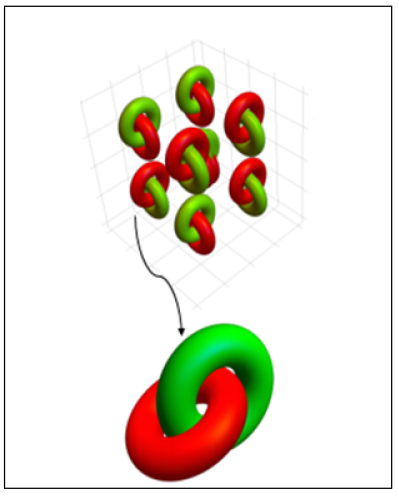
\includegraphics[width=.9\linewidth]{images/nine_ring.png}
  \caption{Nine ring dataset}
  \label{nine_ring_dataset}
\end{subfigure}\hfill
\begin{subfigure}[t]{.45\textwidth}
  \centering
  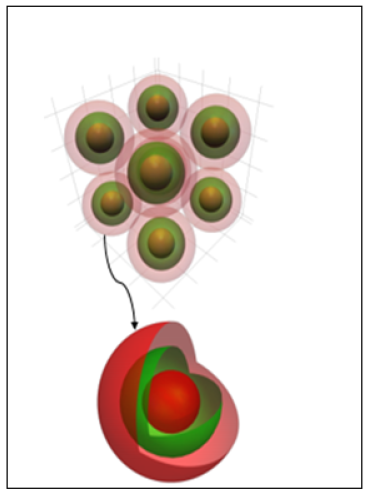
\includegraphics[width=.74\linewidth]{images/nine_sphere.png}
  \caption{Nine sphere dataset}
  \label{nine_sphere_dataset}
\end{subfigure}
\vspace{.2in}
\caption{3 dimensional synthetic datasets with two different classes(Red and Green) used for training MLP}
\label{synthetic_dataset}
\end{figure}

%\begin{figure}
%\begin{tabular}{ccc}
%\bmvaHangBox{\fbox{\parbox{2.7cm}{~\\[2.8mm]
%\rule{0pt}{1ex}\hspace{2.24mm}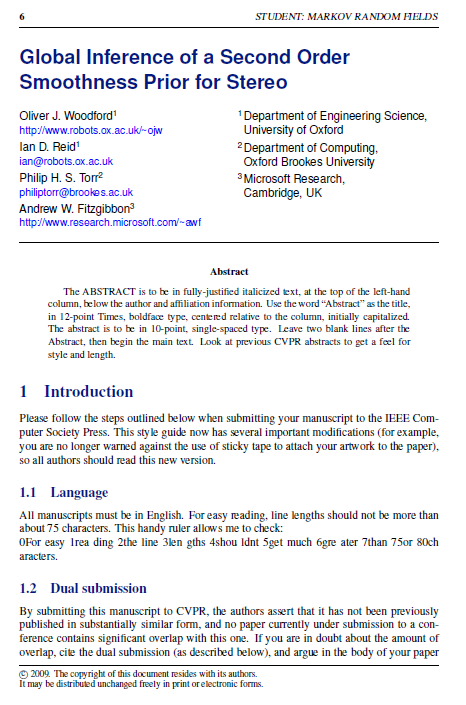
\includegraphics[width=2.33cm]{images/eg1_largeprint.png}\\[-0.1pt]}}}&
%\bmvaHangBox{\fbox{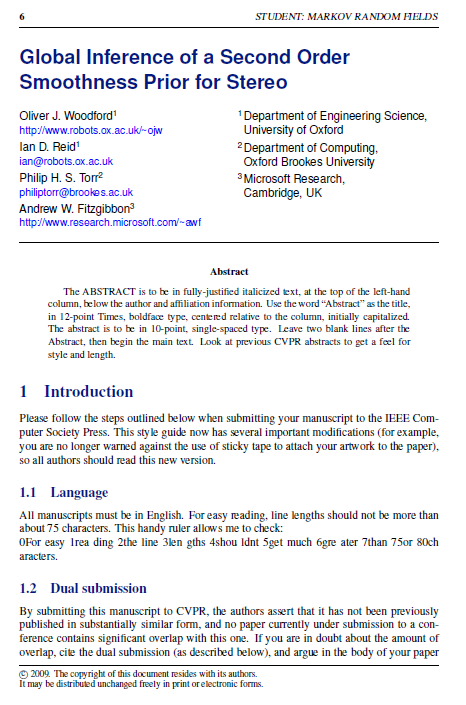
\includegraphics[width=2.8cm]{images/eg1_largeprint.png}}}&
%\bmvaHangBox{\fbox{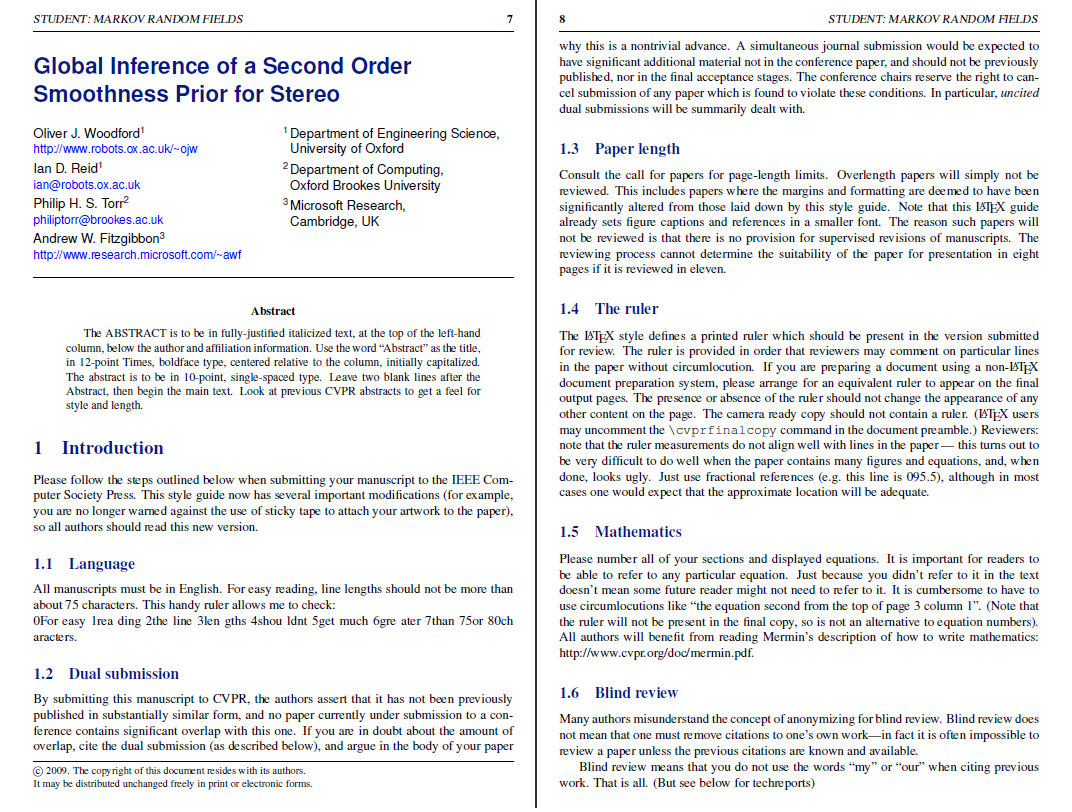
\includegraphics[width=5.6cm]{images/eg1_2up.png}}}\\
%(a)&(b)&(c)
%\end{tabular}
%\caption{It is often a good idea for the first figure to attempt to
%encapsulate the article, complementing the abstract.  This figure illustrates
%the various print and on-screen layouts for which this paper format has
%been optimized: (a) traditional BMVC print format; (b) on-screen
%single-column format, or large-print paper; (c) full-screen two column, or
%2-up printing. }
%\label{fig:teaser}
%\end{figure}

The datasets were converted to gray scale and normalized. No other preprocessing was performed.
\subsection{Design of Layer Transfer Function}
\label{activation_function_design}
The layer transfer function is composed of an affine transformation and a non-linear activation function. In the subsections below, we provide the details of desired characteristics for activation function from a topological point of view.
\subsubsection{Betti numbers and their significance on  layer transfer function}
Betti numbers, denoted as $\beta_k(X)$  are used to quantify the topological complexity of a $d$-dimensional topological space $X$ where $0 \leq k \leq d$. The $0^{th}$ betty number $\beta_0(X)$ is the number of connected components, the first betti number $\beta_1(X)$ is the number of one dimensional holes, the second betti number is the number of two dimensional holes and so on. Figure 6 shows some topological spaces and their corresponding betti numbers. For efficient classification, one needs to transform the original point data cloud, $X$,  from a high dimensional space with large betti numbers to a low dimensional latent representation with $0^{th}$ betti number (number of connected components) equal to the number of classes $K$ and all other betti numbers to zero. As evident from Figure 6, this ensures that each connected component  corresponds to a single class ( either Red or Green) and there are no holes within the connected components. Hence  each connected component is contractible  to a single point. It is easy to find a decision boundary if there are no holes on the manifold formed by samples from a  single class.  In the rest of this document wherever we mention the term  topological complexity, we mean the betti numbers of the topological space.
\subsection{Pruning of Convolutional Neural Network}
\label{network_pruning}
\section{Results}
\section{Conclusion}




%\begin{figure*}
%\begin{center}
%\fbox{\rule{0pt}{2in} \rule{.9\linewidth}{0pt}}
%\end{center}
%   \caption{Example of a short caption, which should be centered.}
%\label{fig:short}
%\end{figure*}


%\begin{table}
%\begin{center}
%\begin{tabular}{|l|c|}
%\hline
%Method & Frobnability \\
%\hline\hline
%Theirs & Frumpy \\
%Yours & Frobbly \\
%Ours & Makes one's heart Frob\\
%\hline
%\end{tabular}
%\end{center}
%\caption{Results.   Ours is better.}
%\end{table}

\bibliography{egbib}
\end{document}
